%!TEX root = DMmidterm.tex

\section{Project}
\label{sec:Project}

%\begin{figure*}[]
%	\begin{center}
%		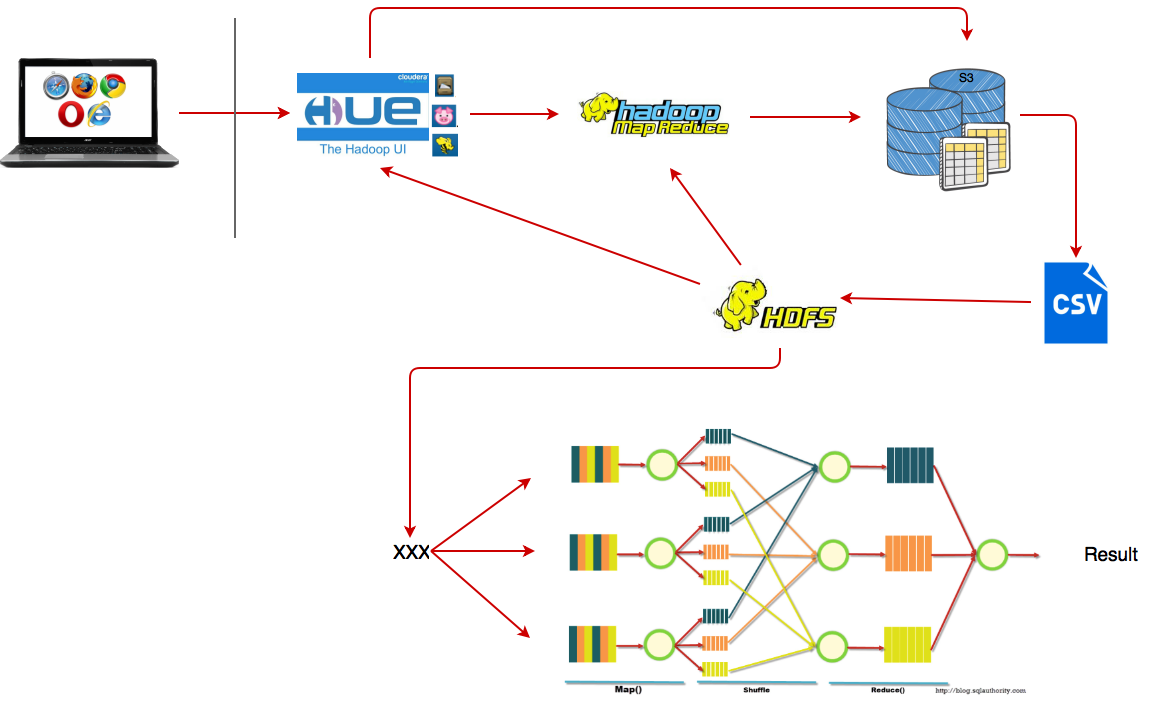
\includegraphics[width=2\columnwidth]{/Users/MariaFerman/Desktop/DC_FinalProject/images/Diagram}
%		\caption{Project Diagram}
%		\label{fig:dataDiagr}
%	\end{center}
%	\vspace{-10pt}
%\end{figure*}

%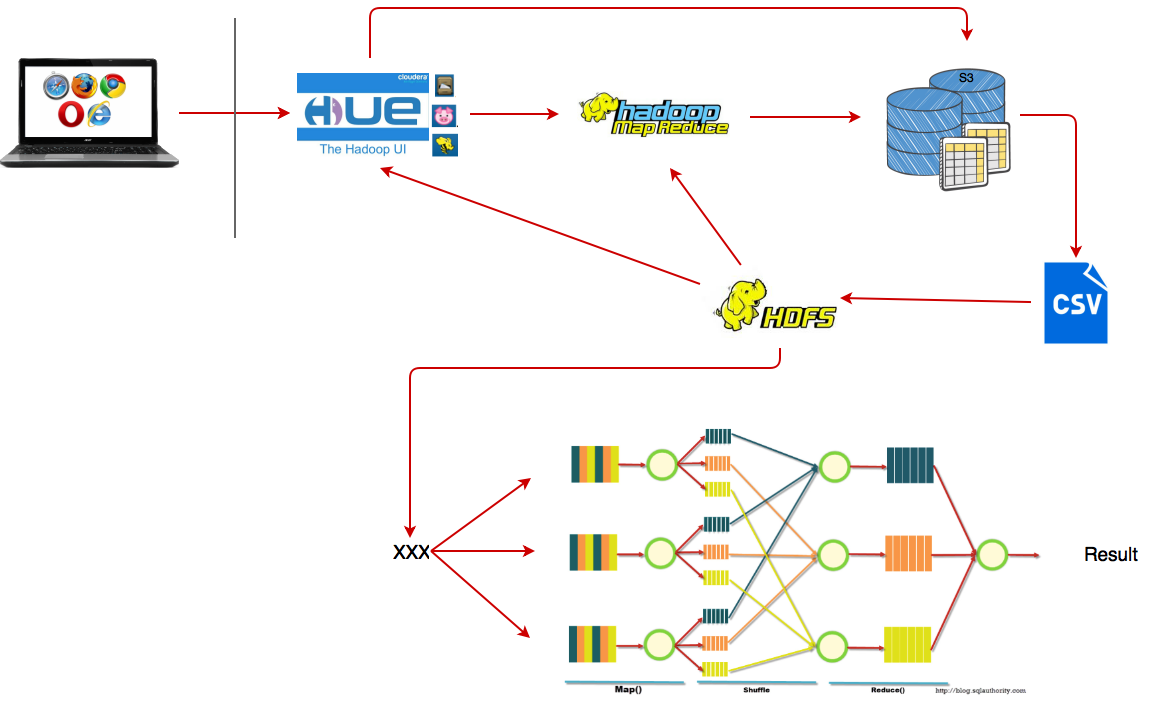
\includegraphics{/Users/MariaFerman/Desktop/DC_FinalProject/images/Diagram}


\subsection{ Dataset}
The dataset gathered for this project comes from the Pacific Climate Impacts Consortium (PCIC) of the University of Victoria. The dataset consist in a series of climate measurements that shows how the climate changes and varies over time. All the measurements were gathered at the same location in the Pacific and Yukon region of British Colombia, Canada.
%The dataset has different networks such as BC Hydro,  environmet Canada, Ministry of transportation among other. 
The dataset is divided by time and stations. The station is the exact location where the data were gathered. 
The dataset will allow us to understand the climate change among time and regions (stations). The resulting analysis of the dataset might help for trend analysis and climate change researches. This information can be used as an input for more complex climate models in order to have accurate climate predictions.

\subsection{Scripts}
To add ...

\subsection{Implementation}
To add ...
In this section we present our implementation of the project.  

Pig To add ...
\begin{figure}[h!]
	\begin{center}
		\includegraphics[width=1\columnwidth]{/Users/MariaFerman/Desktop/DC_FinalProject/images/PigDiagram}
		\caption{Pig Diagram}
		\label{fig:dataDiagr}
	\end{center}
	\vspace{-10pt}
\end{figure}

Hive To add ...
\begin{figure}[h!]
	\begin{center}
		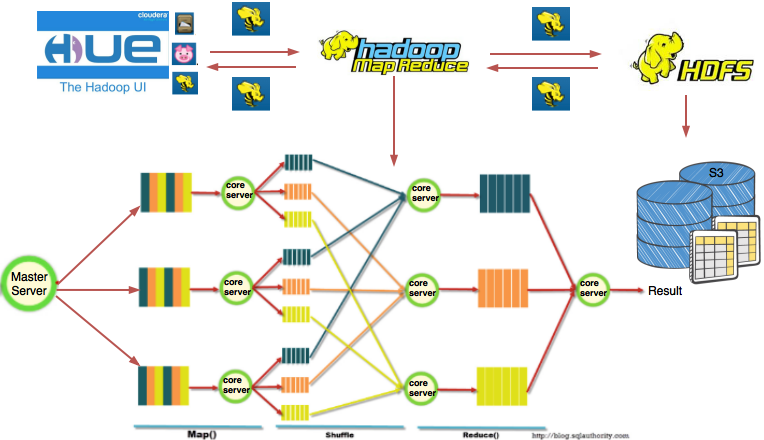
\includegraphics[width=1\columnwidth]{/Users/MariaFerman/Desktop/DC_FinalProject/images/HiveDiagram-2}
		\caption{Hive Diagram}
		\label{fig:dataDiagr}
	\end{center}
	\vspace{-10pt}
\end{figure}


